% Chapter 1

\chapter{Introduction} % Main chapter title
\label{Chapter1} % For referencing the chapter elsewhere, use \ref{Chapter1} 

This chapter presents a brief overview of the present thesis.
First we introduce some basic concept about data and knowledge along with some examples,
then the main contribution is explained with some more in-depth discussion,
followed by the document outline.

\section{Relationship between data and knowledge}

The current amount of digital data produced daily is estimated to be in the realm of 
ZettaBytes ($1~ZB = 10^{12}~GB$) \cite{idc}.
Of this amount, only a small fraction sees actual processing and interpretation,
mainly because while the flow of information is steady, the available resources
devoted to the task are often limited \cite{idc}.
Moreover in some cases the rapidity at which a meaningful interpretation of the 
raw data has to be produced is critical.
Hence, just the plain fact of owning the data does not imply that some useful 
information pattern can be derived from it; in fact the whole discipline of \emph{Data Mining}
was born with the intent of derive \emph{knowledge} that ``we don't know we don't know''.

Most of data mining techniques draw from a variety of other fields like Statistics,
Computer Science, Information Theory and Mathematics just to mention a few.
This discipline rests its theoretical foundation upon the field of \emph{Machine Learning},
the discipline that studies algorithms and techniques that allows a machine
to learn a concept (or an approximation of it) from a set of examples.
These algorithms start from limited evidence and try to build up a general model
by refining an initial \emph{hypothesis}.
Machine Learning is mostly useful when either an exact solution to a very
difficult problem is computationally infeasible or the problem specification
is rather vague or not unambiguously defined, leaving to the algorithm the burden
of exploration.

One of the pivotal concepts of this field is data \emph{representation}.
For the most part, data is collected and stored in unstructured form, e.g. vectors,
and a lot of machine learning techniques are tailored to this representation.
In the last decades some approaches tried to address those problems whose data cannot
be represented in vectorial form or whose representation in this form would cause
information loss.
%----------------------------------------------------------------------------------------

\section{Why structured data}
\label{sec:why}
% ci sono un sacco di dati strutturati
% c'e` la necessita` di applicare machine learning
% se li rappresentiamo come vettori non va bene perche` si perde struttura e piu`
% cresce il mapping piu` trattarlo diventa difficile.

The increasing amount of available structured data has made it necessary to develop
machine learning methods that can effectively deal with it.
More specifically some work has been done to devise methods that could learn
directly from graphs, a very useful kind of \emph{structured data} that sees many
important real-world applications nowadays, encompassing the fields of Computational
Biology, Computer Vision and Natural Language Processing.
For these applications it is natural to collect data that carries an inherent
amount of information concerning its structure.
That is, some data is naturally structured, e.g. molecular graphs or a sentence parse tree,
and represent it in vectorial form will inevitably cause a loss of information about
its structure.
Moreover, adding structural information to a vectorial representation
makes it more complex and consequently more difficult to work with.

Graphs are a structured data form that can represent a great deal of different
information depending on the domain of application.
Graphs have multiple levels of information semantics and each level can have
different connotations, e.g. consider the set of edges, they can represent
different notions of link between two nodes while maintaining the same
representation.
Beside edges, that express a kind of local ``relationship''
information among the nodes, we have information stored at the node level in the
labels, where some qualitative or quantitative data may be present.
At a higher level we have topological information, which can be
viewed like an extended relationship level, and finally the information that can
be derived by looking at the shape of the graph such as notions
of connectivity, density etc.

\subsubsection{Examples}
\label{subsubsec:examples}

Chemical compounds are naturally represented by their molecule; a simple graph
representation of a molecule is given in Figure \ref{fig:chem}.
Most of the benchmark datasets employed in this study contain chemical compounds
represented in a similar way.

\begin{figure}[ht]
    \centering
    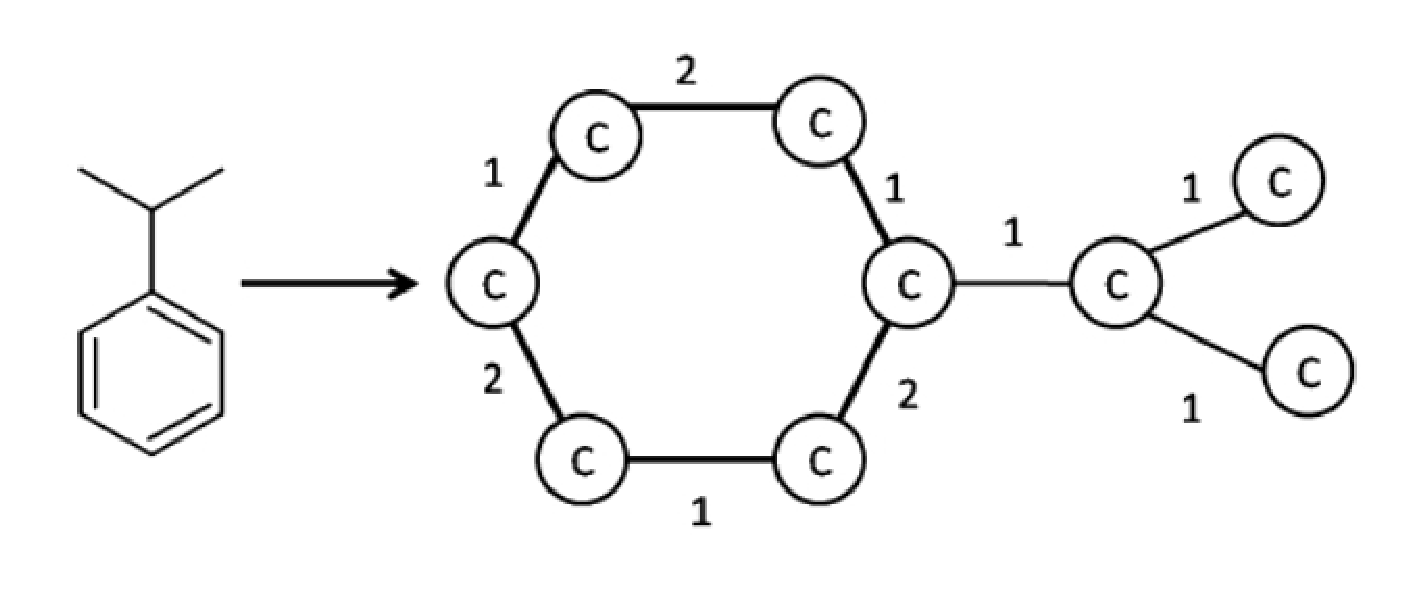
\includegraphics[scale=0.4]{Figures/chcomp}
    \caption{A molecule representation for a chemical compound and its representation
    as a graph; the nodes represent the atoms, the edges represent the chemical bounds and
    are labeled accordingly.}
    \label{fig:chem}
\end{figure}

Graph structured data has proven useful in the classification of non-coding RNA
molecules, modeled as shown in Figure \ref{fig:bio} \cite{nnavarin, conf/psb/KarklinMH05},

\begin{figure}[ht]
    \centering
    \begin{subfigure}{.4\textwidth}
        \centering
        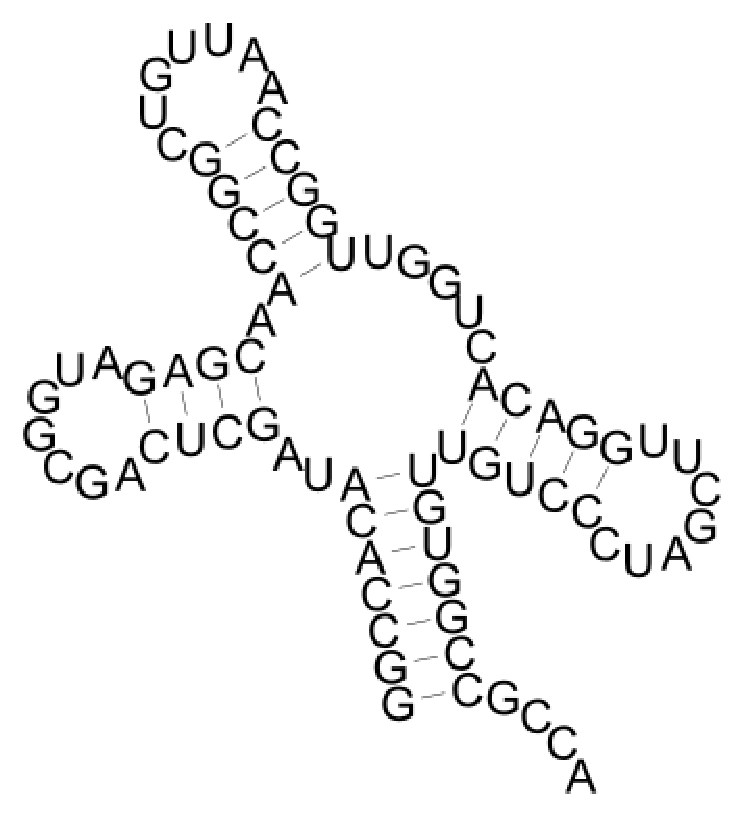
\includegraphics[width=\linewidth]{Figures/rna}
        \label{fig:rna}
        \caption{}
    \end{subfigure}
    \begin{subfigure}{.4\textwidth}
        \centering
        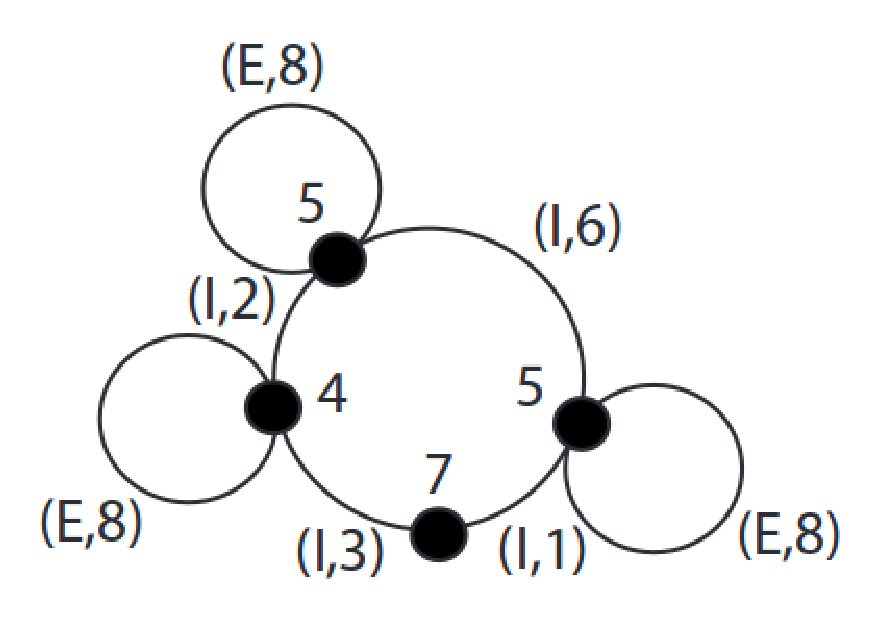
\includegraphics[width=\linewidth]{Figures/ldgrna}
        \label{fig:ldg}
        \caption{}
    \end{subfigure}
    \caption{a) RNA molecule graph representation and b) the same molecule represented
        as a labeled dual graph \cite{conf/psb/KarklinMH05}.}
    \label{fig:bio}
\end{figure}

Natural Language Processing is another field where graph representation is often used
as the basis for elaborate meaning extraction, as is the case for building opinion
lexicon from users review \cite{10.1371/journal.pone.0079294}, see Figure \ref{fig:wordrel}.

\begin{figure}[ht]
    \centering
    \includegraphics[width=.6\linewidth]{Figures/wordrel}
    \caption{Example of graph representation of words relationships in a multilingual
    context \cite{10.1371/journal.pone.0079294}.}
    \label{fig:wordrel}
\end{figure}

In Computer Vision a prominent application that uses graph representation is
the so-called scene understanding or scene modelling task, i.e. a scene is divided
into semantically meaningful areas which can be seen as nodes of a graph whose
edges are the adjacency relations between the areas \cite{journals/corr/abs-1108-4079},
an exemplification of this is given in Figure \ref{fig:scene}.

\begin{figure}[ht]
    \begin{subfigure}{.45\linewidth}
        \centering
        \includegraphics[width=\linewidth]{Figures/scene}
        \caption{}
        \label{fig:scene}
    \end{subfigure}
    \begin{subfigure}{.45\linewidth}
        \centering
        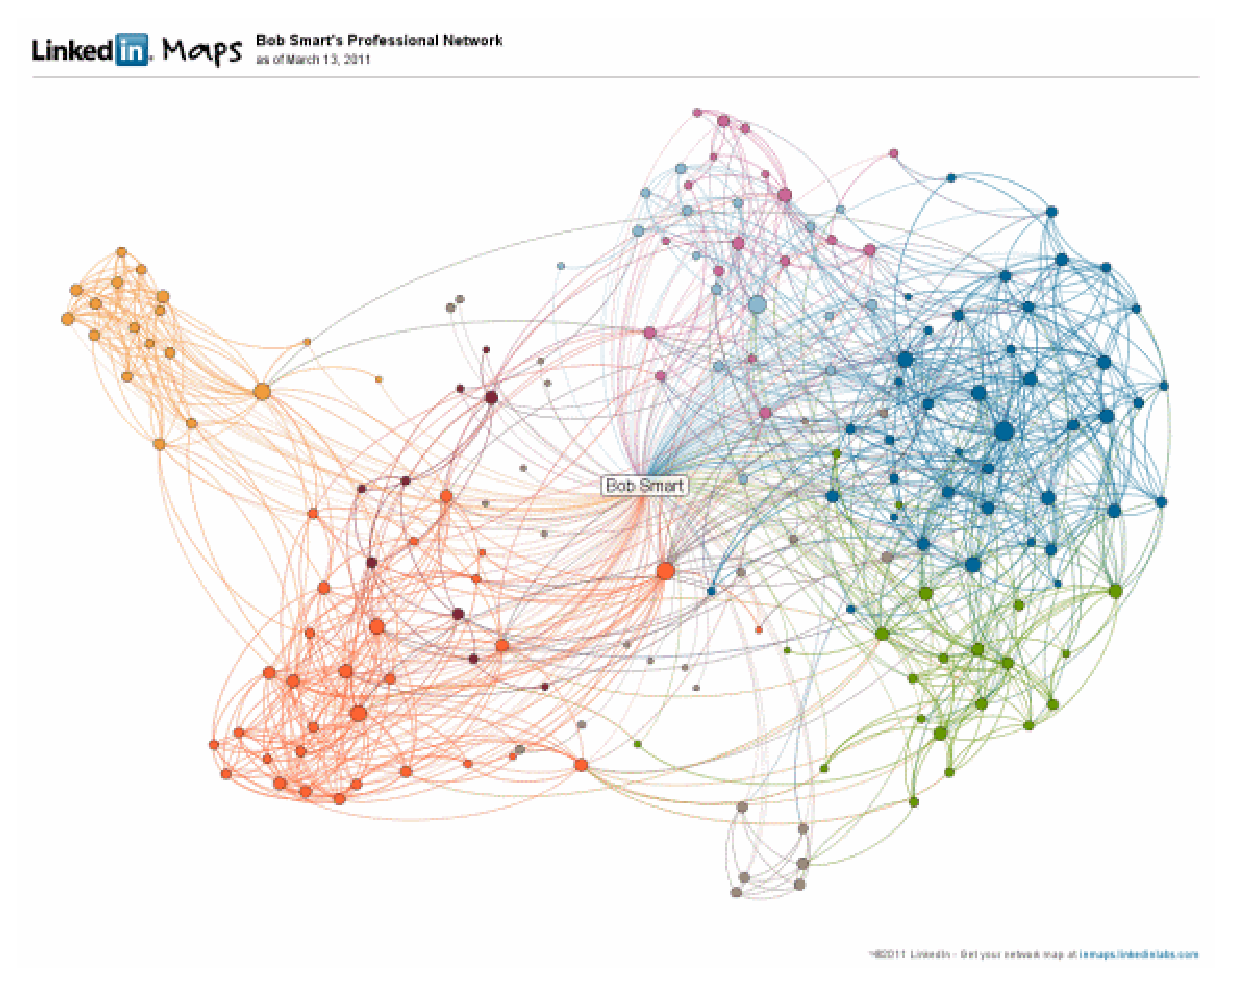
\includegraphics[width=\linewidth]{Figures/linkedin-social-maps}
        \caption{}
        \label{fig:network}
    \end{subfigure}
\caption{a) Scene understanding via graph decomposition in Computer Vision. b)
        LinkedIn's social maps show how a social network graph representation
        can quickly become very complex.}
\end{figure}

Finally, graphs deriving from the inherently structured organization of every social
network can lead to a large number of mining possibilities given the vast
amount of data available \cite{gundecha2012mining}.
Figure \ref{fig:network} shows an example of social network derived from a real-world
application.

%----------------------------------------------------------------------------------------

\section{Graph kernel learning}

Given the wealth of available data, how can we learn from graphs? A first \emph{structure-based}
approach consists in designing an \emph{ad-hoc} vectorial representation for the
particular kind of graphs being considered.
A major downside of this approach is that a renewed effort for the 
design of a new representation is needed every time a new type of data
is encountered.

Another way to address the problem of graph learning is to adapt the existing methods
to work directly on graphs, thus allowing the exploitation of the existing techniques.
Some recently proposed works \cite{DBLP:conf/sdm/MartinoNS12, NIPS2009_3813}
embed graph specific knowledge into well established \emph{kernel methods}
that, given the inherent decoupling between the data representation and the learning
algorithm that they provide (more on Section \ref{subsec:introkm}), represent a
more general approach.

This thesis focuses on these kernel methods, and their use on a binary classification
task in a supervised setting that is, a task in which the machine learning algorithm
has to separate (classify) two sets of already labelled samples (hence ``supervised'').
In the following sections we assume to be operating in this scenario.

\subsection{Kernel methods}
\label{subsec:introkm}

Kernel methods are a collection of techniques that rely on an implicit representation
of the data and a well defined measure of similarity between samples to perform
the learning task.
These methods have two main components: a domain specific function to compute the
samples similarity score, called \emph{kernel function}, and a general purpose
learning algorithm, often called \emph{kernel machine}, to combine the information provided by the
kernel function in order to separate the samples.

Kernel functions implicitly map examples in a high dimensional space, commonly
referred to as \emph{feature space}, and define the similarity score as a dot
product in this space.
Specific domain knowledge gets embedded in the learning process through the definition
of the kernel function that becomes the only interface between the data
and the learning algorithm.
The explicit representation of the feature space is never accessed by the algorithm
that refers to it only implicitly through the kernel function.
This is commonly known as the \emph{kernel trick} and the reason behind it is 
that computing the dot product for each pair of samples in a high dimensional space
would be infeasible but can be avoided thanks to the kernel function since they are
equivalent (Section \ref{subsec:kernelfunc}).

Kernel machines are learning algorithms that employ the similarity measures defined
by kernel functions to find a linear separator in a high dimensional feature space
since it is usually easier; once a separator has been found, it is mapped back
to the original input space from where the data was generated.
One of the most adopted methods is the Support Vector Machine (SVM) \cite{Cortes&Vapnik:1995}
which is a binary classifier that tries to find a separator that maximizes the \emph{margin}
between two sets of labelled samples that is, the distance between the separator and the
nearest sample of each class.
SVMs employ the samples pairwise distance as their similarity measure.

\subsection{Hyper-parameter selection}
\label{subsec:hyper1}

Most learning methods have parameters that need tuning, i.e. in order to achieve
good generalization performances each value has to be selected from a set of
possible choices according to a performance measure.
These parameters, often referred to also as \emph{hyper-parameters}, define a
\emph{parameter space} characterized by their number, and by the size and type
of their domains.
This space can be potentially infinite and it is usually highly non-convex, making
the search for a global optimum very hard, if any exists.

For this reason the selection procedure often involves a limited search on the parameter space
that is, a set of values for each parameter is fixed, possibly after a discretization,
and all the combinations are tested to find the best one.
However, in order to be useful the sampling on the parameter space needs to be adequate:
even with a heuristic approach the complexity of this search can still be daunting because
it depends on the number of parameters.

In the context of kernel learning hyper-parameters can be found on two levels:
parameters relative to the kernel function and parameters that belongs to the
kernel machine (solver).
The parameters of the former typically influence the feature space being generated,
directly affecting the expressiveness of the similarity measure, i.e. the ability
to discern between two different samples.
The parameters of the solver are usually employed as regularization factors,
as is the case for the SVM, where its only hyper-parameter is used to balance the trade-off between a good
(generalizing) separator and empirical error.
Once the solver has been chosen, the parameter space is determined by the kernel
hyper-parameters hence, the kernel choice can greatly affect the computational
performances of the whole approach.
Moreover, often the kernel has to be selected in a similar way, thus increasing the
computational burden even more.

\subsection{Validation procedures}
The learning process is composed of two main phases, the training phase and
the test phase.
Briefly, in the training phase a model is built trying to approximate a concept, its performances
are then assessed during the test phase.
Each phase employs a different set of data, training data and test data respectively,
that is sampled from the original dataset.
Hyper-parameter values can deeply affect these two phases, in particular
because they determine which hypotheses are selected by the learning algorithm.
There are two main factors that are influenced by the values selected for the
hyper-parameters.

On one hand we have \emph{overfitting}, which happens when the hypothesis
(model) returned by the training phase is able to correctly classify the training data
but performs poorly on new instances that get presented to it, i.e. the test data.
This can happen because the selected hyper-parameter values render the model so
complex that it fits to spurious properties of the training data.

On the other hand we have \emph{underfitting} which consists in the hypothesis skewing
in a direction that makes it unable to grasp the full complexity of the data resulting
in a high classification error even on the training data.
This can be due to the model being too simple because of the chosen parameter values. 

To find the optimal balance between these two factors, typically hyper-parameter
selection is performed employing a \emph{validation set}, that is a fixed subset of the
data left out from the training phase and used to validate the performances of a
model built according to a given set of values for the parameters.
In this case the validation set coincides with the test data.
To reduce the bias, i.e. the distortion, deriving from the fixed selection of
the validation set, a k-fold cross-validation technique is employed: the
data is split into $k$ subsets, $k-1$ become the training set while the last one
is used as the validation set; this procedure is repeated $k$ times, with the
validation set being a different one of the $k$ subsets during each iteration
(\emph{fold}).

This way the best performing model built according to a set of parameter values
is selected, which is equivalent to select the best set of parameter values.
This process is still prone to overfitting because, due to the way cross-validation
is performed, the final model gets trained and validated on the same
data.

\subsubsection{Nested cross-validation}
A remedy to the possible overfitting deriving from a cross-validation,
the so-called nested k-fold cross validation is employed.
This technique consists in two k-fold cross-validation nested one within the other.
In the outer loop the whole dataset is split in $k$ subset, one of which becomes the
\emph{test set}.
The remaining training data is then used to perform a regular k-fold cross-validation
whose selected model is trained again on the whole training set and finally evaluated
on the test set.
This technique ensures that the test set is completely left out from the training
process so that the performance estimation is independent from the training data.
The performances estimated on the $k$ obtained models are then averaged and represent
an unbiased performance estimate of the best performing model given the available data.

%\subsection{Proposed solution}
\section{Thesis contribution}
% more detail
% relevance
The task of estimating a model performance is essential in machine learning
but can become very onerous to perform, especially when employing a nested 10-fold
cross-validation technique, 10 being usually a reasonable value for $k$, which
increases the computational times a couple of orders of magnitude with respect
to a single training phase.
Moreover the size and shape of the (finite) parameter space considered while performing
hyper-parameter selection will directly impact on the overall time required to
obtain the desired results.

% problem
% kernel learning typically has a number of params to select
% graph kernel learning more so
% single kernel approach test each kernel ie function+params in isolation
% this can be a problem because kernel computation tends to be heavy.
% so a lot of kernels = a lot of time

Kernel learning methods needs to select the optimal values for a number of parameters
belonging both to the kernel function and to the kernel machine of choice.
Kernel function parameters shape the underlying feature space thus greatly affecting
the resulting kernel performances. Hence the number of values to select from has
to be sized in order to allow a good sampling.
With the standard approach each kernel, i.e. the combination of a kernel function
and a set of parameter values, has to be computed and tested individually and this can
further slow down hyper-parameter selection.
This is particularly true for graph kernel learning, since graph kernels are usually
computationally demanding (Section \ref{subsec:graphk}).

% sol

% intro mkl
A different approach, called \emph{multiple kernel learning} (MKL), has been
developed to allow the combination of different kernels into a single learning phase.
This family of methods typically tries to find the best (non) linear combination between the
given kernels, to increase the individual performances and implicitly perform the
kernel selection in a data driven way.
This approach has been developed with the initial aim to be employed with a small
number of independent and carefully designed kernels in order to beat simpler combination
such as the average.
Recently a second approach has been emphasized that is, combine a large set of possibly
weak kernels with the intended purpose of boosting the overall accuracy.
From the numerous implementations available in literature \cite{journals/jmlr/GonenA11},
we want to mention EasyMKL, a recently proposed state-of-the-art MKL implementation
\cite{aiolli2015easymkl} with a linear complexity bound w.r.t. the input size.
This algorithm is an \emph{optimization based} MKL implementation with a strong
theoretical background (Section \ref{subsec:easymkl}) and was selected to be part
of the this work.

In this study we propose a methodology to perform graph kernel learning avoiding
the process of kernel hyper-parameter selection, reducing the overall time
required to do the model performance estimation without significantly losing
predictive performances.
Employing EasyMKL combination capabilities from a different perspective, we
perform the learning task employing at once all the kernels that would have been
individually computed according to a kernel parameters grid (Section \ref{subsubsec:grid}).
Therefore we achieve a consistent reduction of the hyper-parameters to validate, since
eliminating all the kernel function parameters from the selection process, only those of the
kernel machine remain.

% results

The obtained results show on average a significant decrease in computational times across the
considered datasets while the predictive performances remain comparable when not
above the selected baseline methods.
Moreover, the proposed methodology can be generalized to consider multiple kernel functions.

With this approach the whole process of hyper-parameter selection has been streamlined and
lifted from the kernels to the learning machine, effectively eliminating the need to test each
kernel in isolation.

%----------------------------------------------------------------------------------------

\section{Thesis outline}
This document is organized as follows: in Chapter \ref{Chapter2} we delve into
the background details that are necessary to fully understand the proposed idea;
we cover the basics of machine learning and kernel methods and see some examples
of kernel combination techniques.
The main ideas behind this work are exposed in Chapter \ref{Chapter3} where we
discuss in detail our approach, the conceptual steps involved and the solutions
to the problems encountered.
Chapter \ref{Chapter4} covers the experimental part of the thesis, where we present
our results and finally in Chapter \ref{Chapter5} we draw conclusions and explain
how some ideas proposed here can be further explored.

%----------------------------------------------------------------------------------------

% vim: spell spelllang=en_gb
